\documentclass[a4paper,10pt]{article}
\usepackage[dvips]{color,graphicx}
\usepackage[dvips, bookmarks, colorlinks=false]{hyperref}


%opening
\title{Math508 Homework 12}
\author{Yu Huang}
\date{2007-04-26}

\begin{document}

\maketitle

\begin{abstract}
Continuous state space Filtering
\end{abstract}

\section{Problem 3}
\subsection{Solve integral by Riemann sum}
The difficult part is how to integrate the probability function. The idea is to replace the integral with a Riemann sum over the support where probability mass is not trivial. Based on the model, the signal $X_n$ is concentrated around 7 with small variance. As the sequence progresses, the general trend of $X_n$ goes upward though it's slow (due to the fact $X_{n+1} = 1.004X_n + 0.06X_nVn$).

\begin{equation}
\int_a^b f(x) dx = \sum_{x_i=a}^{x_i<b} f(x_i) \Delta x
\end{equation}


The support we pick is $[-20, 30]$. Different $\Delta x$ were tried. Smaller $\Delta x$, smaller mean squared error.


Figure~\ref{f1} is $\Delta x=0.15$. Figure~\ref{f2} is $\Delta x=0.34$. $\Delta x=0.5, 0.35$ could result in zero float division in normal density.


\subsection{algorithm of partical filter or sequential importance resampling}
The idea is 
\begin{equation}
E(F(\mathbf{X}_t)) = \int F_t(\mathbf{X}_t) \pi_t(\mathbf{X}_t|\mathbf{Y}_t) d\mathbf{X}_t = \int F_t(\mathbf{X}_t) \frac{\pi_t(\mathbf{X}_t|\mathbf{Y}_t)}{P(\mathbf{X}_t|\mathbf{Y}_{t-1})} P(\mathbf{X}_t|\mathbf{Y}_{t-1}) d\mathbf{X}_t
\end{equation}


\begin{eqnarray}
\pi_t(\mathbf{X}_t|\mathbf{Y}_t) = \frac{P(X_t, Y_t, \mathbf{X}_{t-1}|\mathbf{Y}_{t-1})}{P(Y_t)} \\
P(X_t, Y_t, \mathbf{X}_{t-1}|\mathbf{Y}_{t-1}) = P(Y_t|X_t)P(X_t|\mathbf{X}_{t-1})P(\mathbf{X}_{t-1}|\mathbf{Y}_{t-1}) \\
P(\mathbf{X}_{t-1}|\mathbf{Y}_{t-1}) = \pi_t(\mathbf{X}_{t-1}|\mathbf{Y}_{t-1}) \\
\pi_t(\mathbf{X}_t|\mathbf{Y}_t) = \frac{P(Y_t|X_t)P(X_t|X_{t-1})\pi_t(\mathbf{X}_{t-1}|\mathbf{Y}_{t-1})}{P(Y_t)}
\end{eqnarray}

The proposal distribution is $P(\mathbf{X}_t|\mathbf{Y}_{t-1}) = P(X_t|X_{t-1})\pi_t(\mathbf{X}_{t-1}|\mathbf{Y}_{t-1})$. The importance weight is $\pi_t(\mathbf{X}_t|\mathbf{Y}_t)/P(\mathbf{X}_t|\mathbf{Y}_{t-1}) = P(Y_t|X_t)/P(Y_t)$. As $P(Y_t)$ could be regarded as constant, the weight is just $P(Y_t|X_t)$.

For $t=0$, the proposal distribution is $P(X_0)$ and the importance weight is $P(Y_0|X_0)$.

The algorithm looks like
\begin{itemize}
\item sample $x_t^i$ from $P(X_t|X_{t-1})$ for $i=1,...,n$
\item weight each sample by $w(x_t^i) = P(Y_t|x_t^i)$
\item estimate is $\hat{x}_t = \sum_{i=1}^n x_t^i*w(x_t^i)$. Note: it's not the $x_t^i$ with maximum weight cuz it simply picks the one closest to the observation, $Y_t$.
\item resample from $\{x_t^1, ..., x_t^n\}$ with probability proportional to $w(x_t^i)$ to produce a random sample $\{x_t^{*1}, ..., x_t^{*n}\}$
\end{itemize}

Figure~\ref{f3} is the result by SIR and it's pretty good (mse=0.4908) with 10000 samplings each iteration.

\section{Figures}

\begin{figure}
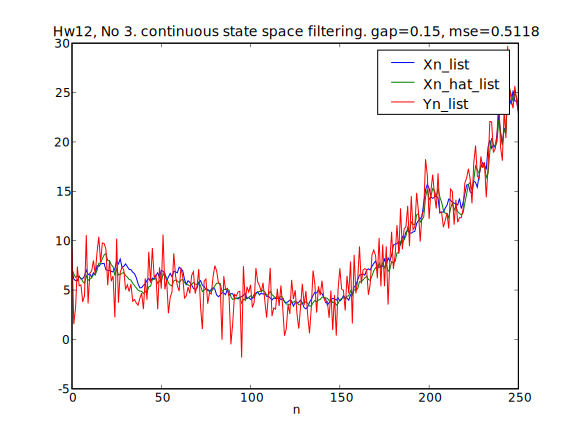
\includegraphics[width=1\textwidth]{hw12_3_gap_0_15.eps}
\caption{}\label{f1}
\end{figure}

\begin{figure}
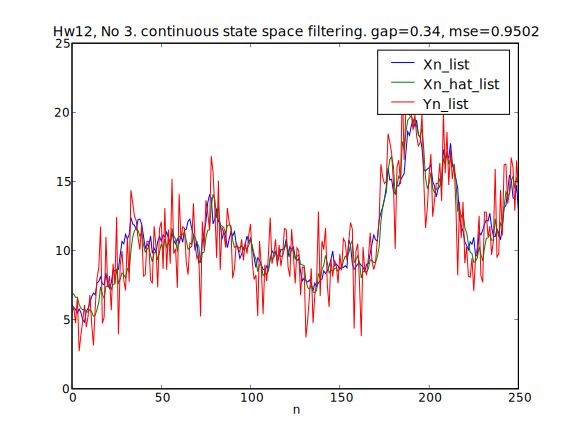
\includegraphics[width=1\textwidth]{hw12_3_gap_0_34.eps}
\caption{}\label{f2}
\end{figure}

\begin{figure}
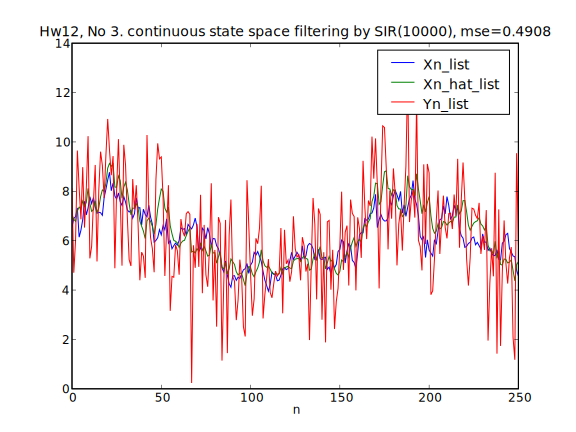
\includegraphics[width=1\textwidth]{hw12_3_SIR_10000.eps}
\caption{}\label{f3}
\end{figure}

\end{document}
